\section{An Introduction to \acs{NMR}}

\subsection{A Brief History}
Since its conception almost 80 years ago, \ac{NMR} has become a ubiquitous
technique in chemistry, biochemistry and numerous other disciplines, thanks to
the unique insights into chemical structure and dynamics that it
can provide.
The origins of the subject can be traced back to 1945, when independent work by
Felix Bloch on water~\cite{Bloch1946} and Edward Purcell on
paraffin~\cite{Purcell1946} gave rise to the first illustrations of nuclear
magnetic resonances in condensed phases. The two hadn't met before their
respective papers were published with about a month's
separation~\cite{Becker1993}. Both received the Nobel Prize in Physics in 1952
``for their development of new methods for nuclear magnetic precision
measurements and discoveries in connection therewith''~\cite{Nobel1952}. A
notable mention should also be given
to Yevgeny Zavoisky, the father of the related field of electron paramagnetic
resonance, who probably observed NMR as far back as 1941~\cite{Eaton1998}. Alas,
he dismissed
his results as irreproducible. A few years subsequently, works investigating
\ac{NMR} spectra from compounds containing nuclei such as \ch{^{63}Cu},
\ch{^{65}Cu}, \ch{^{31}P}, \ch{^{14}N}, and \ch{^{19}F} led to an
understanding of the \emph{chemical shift}, a phenomenon in
which nuclei in different chemical environments exhibit
non-identical resonant frequencies~\cite{Knight1949, Proctor1950,
Dickinson1950}.  Chemists regarded these findings with great
interest, as they suggested that \ac{NMR} could give insights into molecular
structure.

Russell Varian\,---\,founder of \textsc{Varian Associates} along with his brother
Sigurd\,---\,
secured the first patent for a commercial \ac{NMR} machine, with
a \qty{30}{\mega\hertz} spectrometer following soon after. The first
spectrometers functioned by gradually varying the magnetic field strength,
causing spins to come into resonance at different times, in a process referred
to as continuous wave spectroscopy. Richard Ernst and
Weston Anderson, working at \textsc{Varian} at the time, proposed an alternative
method: pulsed \ac{FT} spectroscopy~\cite{Ernst1966}. This was not seen as a
fruitful endeavour by the company, largely because of the very long time it
took to digitise the signal, and subsequently compute its FT~\cite{Freeman2015}.
Instead, the first commercial pulsed \ac{FT} spectrometer was produced by
\textsc{Bruker Corp.} in 1969, which revolutionised NMR. The innovation emerged
shortly after Cooley and Tukey's introduction of the \ac{FFT}
algorithm~\cite{Cooley1965}, which incentivised the development of the pulsed
\ac{FT} approach.

The concept of \ac{2D} \ac{NMR} spectroscopy was proposed by Jean Jeener in
1971~\cite{Jeener1971, Jeener2016}, which Ernst and co-workers showcased a few
years later in the form of a \ac{COSY} experiment~\cite{Aue1976a}. The use of
multiple dimensions to spread out signals enabled vastly more complex
structures to be studied. In 1985, the first protein assignment by
\ac{NMR}\,---\,using \ac{COSY} and \ac{NOESY} experiments\,---\,was reported
by Kurt W\"uthrich and co-workers~\cite{Williamson1985}. Over time, extensive
developments in techniques for biomolecular systems have occurred, including
the creation of 3D and 4D ``triple resonance'' experiments~\cite{Marion1989,
Kay1990}, as well \ac{TROSY} experiments~\cite{Pervushin1997} for the study of
large proteins.

\ac{NMR}'s significance as an analytical tool is evidenced by Nobel Prizes in
Chemistry being awarded for work in the field on two separate occasions, on top
of the 1952 Physics Prize. First,
Ernst received the prize in 1991 ``for his contributions to the development of
the methodology of high resolution \acl{NMR}"~\cite{Ernst1992}. In 2002,
W\"uthrich was recognised ``for his development of \acl{NMR} for determining
the three-dimensional structure of biological macromolecules in
solution"~\cite{Wuthrich2003}.

\subsection{The Bloch Model}

\ac{NMR} relies on an intrinsic property of \correction{nuclei with an odd number of
protons and/or neutrons}\label{corr:prot-neut} called \textit{spin}
which, along with orbital angular momentum \correction{and molecular rotation, is one of
the sources}\label{corr:mol-rot} of angular momentum in quantum mechanics.
The angular momentum associated with a nuclear spin is characterised by the
quantum number $I \in \lbrace 0, \nicefrac{1}{2}, 1, \nicefrac{3}{2}, \cdots
\rbrace$. Spin-\nicefrac{1}{2}
nuclei are the most commonly studied in \ac{NMR}, as those with $I >
\nicefrac{1}{2}$ often have very short-lived excited states due to electric
quadrupole effects. A rigorous description of \ac{NMR} requires the application
of quantum mechanics, with many excellent texts on the subject available to
suit newcomers and experts alike; notable examples include the
following citations (in approximate order of complexity):
~\cite{Hore2015,Levitt2007,Cavanagh2007,Goldman1988,Abragam1961,Kuprov2023}.
Despite this, a basic
appreciation can be gained using the Bloch (vector) model, a semi-classical
description of the simplest possible system to study: a ensemble of
isolated, identical spin-$\nicefrac{1}{2}$ nuclei~\cite[Chapter 1]{Hore2015}.
The Bloch model becomes inadequate when more complex spin systems are
considered, featuring non-identical spins which interact through mechanisms
such as scalar couplings (commonly referred to as J-couplings), dipolar
couplings etc. However, it provides valuable insights into the basic principles
of \ac{NMR}, including the form that a typical dataset acquired by an
experiment takes.

The nuclear spin angular momentum $\symbf{I} \in \mathbb{R}^3$ is a
vector\footnote{
    In most of this work, vectors are expressed as lower-case
    bold letters and matrices/multidimensional arrays are expressed as
    upper-case bold letters. However, in this section notation
    frequently encountered in the literature is used, which violates this.
} with squared magnitude
\begin{equation}
    \symbf{I}^2 = \symbf{I} \cdot \symbf{I} = \hbar\correction{^2} I (I + 1),
  \label{eq:I-squared}
\end{equation}
where $\hbar \coloneq \nicefrac{h}{2 \pi}$ is the reduced Planck constant
(\qty{1.055e-34}{\joule\second}). While it
is not possible to specify multiple components of the angular momentum
simultaneously in accordance with the uncertainty principle, it is possible to
specify one of these along with $\symbf{I}^2$. Conventionally, this is chosen
to be the $z$-component, for which
\begin{equation}
  I_z = \hbar m \quad \forall
    m \in \lbrace -I, -I+1, \cdots, I - 1, I \rbrace.
  \label{eq:Iz}
\end{equation}
\cref{eq:Iz}
implies that the magnitude of the $z$-component may only adopt certain discrete
values (i.e. it is quantised). A nucleus \correction{with
spin}\label{corr:with-spin} has an associated
\textit{magnetic moment}, given by\footnote{
    In the context of solution-state \ac{NMR}, $\gamma$ is often replaced with
    $(1-\sigma)\gamma$, where $\sigma$ is a unitless quantity that accounts for
    chemical shift.
}:
\begin{equation}
  \symbf{\mu} = \gamma \symbf{I} \implies \mu_z = \gamma I_z = \gamma \hbar m.
\end{equation}
$\gamma \in \mathbb{R}$ is a proportionality constant called the
\textit{gyromagnetic ratio}, which is dependent on the nucleus of interest.
\Cref{tab:nuclei} provides the gyromagnetic ratios for some low-mass
nuclei commonly encountered in \ac{NMR}, along with some which
\correction{do not possess spin}\label{corr:no-spin}
and are therefore inert in the context of \ac{NMR}.

\begin{table}
    \begin{center}
        \begin{tabular}{ c c c c }
            \toprule
            Nucleus & $I$ & $\gamma (\si{\per \tesla \per \second})$ & Relative Abundance (\%) \\
            \midrule
            \ch{^{1}H} & \nicefrac{1}{2} & \num{2.6752e8} & 99.9885 \\
            \ch{^{2}H} & 1 & \num{4.1066e7} & 0.0115 \\
            \ch{^{6}Li} & 1 & \num{3.9371e7} & 7.59 \\
            \ch{^{7}Li} & \nicefrac{3}{2} & \num{1.0398e8} & 92.41 \\
            \ch{^{12}C} & 0 & - & 98.93 \\
            \ch{^{13}C} & \nicefrac{1}{2} & \num{6.7279e7} & 1.07 \\
            \ch{^{14}N} & 1 & \num{1.9329e7} & 99.636 \\
            \ch{^{15}N} & \nicefrac{1}{2} & \num{-2.7114e7} & 0.364 \\
            \ch{^{16}O} & 0 & - & 99.756 \\
            \ch{^{17}O} & \nicefrac{5}{2} & \num{-3.6276e7} & 0.038 \\
            \ch{^{19}F} & \nicefrac{1}{2} & \num{2.5176e8} & 100 \\
            \ch{^{31}P} & \nicefrac{1}{2} & \num{1.0833e8} & 100 \\
            \bottomrule
        \end{tabular}
    \end{center}
    \caption[
        Statistics related to a number of nuclei which are regularly-encountered in \acs{NMR}.
    ]{
        \correction{
            Statistics related to a number of nuclei which are
            regularly-encountered in \acs{NMR}.
            Also listed are common nuclei which do not possess spin.
            The gyromagnetic ratios were determined by obtaining the relevant
            nuclear magnetic dipole moments $\mu$ in units of nuclear magneton
            $\mu_{\text{N}}$~\cite{Stone2019},
            and applying the equation $\gamma = \nicefrac{\mu \mu_{\text{N}}}{I \hbar}$,
            where $\mu_{\text{N}} =
            \qty{5.0507837461e-27}{\joule\per\tesla}$~\cite{Tiesinga2021}).
        }
    }
    \label{tab:nuclei}
\end{table}

Without the presence of an external magnetic field, the different nuclear spin
states are degenerate. However, once a magnetic field is applied, the
\emph{Zeeman effect} is observed, whereby the relative energies of the
different states diverge. The energy of a given magnetic moment relative to its
zero-field energy is given by
\begin{equation}
  E = - \symbf{\mu} \cdot \symbf{B}_0,
\end{equation}
where $\symbf{B}_0 \in \mathbb{R}^3$ is the magnetic field vector. In \ac{NMR}
it is conventional to define the external field as directed along the
laboratory $z$-axis, such that $B_{0,x} = B_{0,y} = 0$ and $B_{0,z} = B_0$
where $B_0$ is the magnetic field strength. The energies of the individual spin
states are therefore (\cref{fig:energy_levels})
\begin{equation}
  E_m = - \gamma I_z B_0 = -m \hbar \gamma B_0.
\end{equation}
\begin{figure}%
    \centering%
    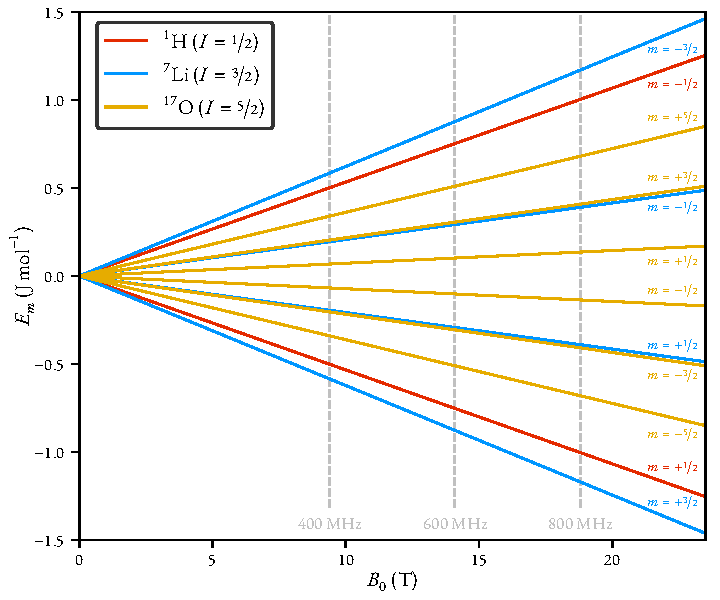
\includegraphics{energy_levels/energy_levels.pdf}%
    \caption[%
        The variation of energy of the spin states of \ch{^1H},
        \ch{^7Li}, and \ch{^{17}O} with external magnetic
        field strength.
    ]{%
        The variation of energy of the spin states of \ch{^1H},
        \ch{^7Li}, and \ch{^{17}O} with external magnetic
        field strength ($B_0$) up to \qty{23.5}{\tesla}, which is
        approximately the strength of a \qty{1}{\giga \hertz} \ac{NMR} magnet.
        Three common field strengths for commercial NMR magnets are indicated:
        \qty{9.40}{\tesla} (\qty{400}{\mega\hertz}), \qty{14.10}{\tesla}
        (\qty{600}{\mega\hertz}), and \qty{18.79}{\tesla}
        (\qty{800}{\mega\hertz}). \correction{Note the relative ordering of the spin states
        for \textsuperscript{1}H and \textsuperscript{7}Li (with positive
        $\gamma$) versus \textsuperscript{17}O (with negative  $\gamma$).}
    }%
    \label{fig:energy_levels}%
\end{figure}%
\ac{NMR} samples comprise a vast ensemble of equivalent spin systems, and it is
the macroscopic properties of the sample that are observed.
At thermal equilibrium, the various spin states will be disproportionately
populated\,---\,albeit to a meager extent due to the small
relative energies involved\,---\,in accordance with the Boltzmann
distribution, with lower energy states being more heavily populated. For
example, an ensemble of
non-interacting spin-$\nicefrac{1}{2}$ nuclei with $\gamma > 0$, such as
\ch{^1H}, will have a more populated $m = +\nicefrac{1}{2}$ (\textalpha) state,
relative to the $m = -\nicefrac{1}{2}$ (\textbeta) state.  Due to the
population imbalance, the ensemble acquires a net (bulk) magnetic moment
$\symbf{M}$, given by the sum of all the individual spin moments:
\begin{equation}
    \symbf{M} = \sum\limits_{s=1}^{S} \symbf{\mu}_s,
\end{equation}
where $S \gg 1$ is the number of spins in the ensemble.
At equilibrium, the $x$- and $y$-components of the bulk magnetisation are zero:
\begin{equation}
    \sum_{s=1}^{S} \mu_{x,s} = \sum_{s=1}^{S} \mu_{y,s} = 0,
\end{equation}
such that the bulk magnetisation is collinear with the field direction, with a
magnitude $M_0$.
\correction{By invoking the \emph{high temperature approximation}\footnote{
        \correction{
            \cref{eq:M0} is arrived at under the assumption that
            $\nicefrac{m\hbar\gamma B_0}{k_{\text{B}} T} \ll 1$. Given typical
            values of $\gamma$ ($\approx\!\!\qty{1e8}{\per\tesla\per\second}$) and
            $B_0$ ($\approx\!\!\qty{10}{\tesla}$), the implicit requirement for
            the temperature to be sufficiently large is virtually always
            adhered to in solution-state \ac{NMR}.
        }\label{fn:corr-high-temp}
    }, $M_0$ may be expressed as~\cite[Section 1.1]{Cavanagh2007}:
}\label{corr:high-temp}
\begin{equation}
    M_0 \approx \frac{S \gamma^2 \hbar^2 B_0 I (I + 1)}{3 k_{\text{B}} T},
    \label{eq:M0}
\end{equation}
where $k_{\text{B}}$ is the Boltzmann constant
(\qty{1.381e-23}{\joule\per\kelvin}),
and $T$ is the sample temperature. To maximise experiment sensitivity, it is
desirable to
utilise nuclei with high natural abundance (affecting $S$ for a given sample
concentration), and high
gyromagnetic ratio. Along with other favourable attributes such as its ubiquity
in organic molecules, \ch{^1H} is therefore by far the most popular nucleus to
study using \ac{NMR}, at least in solution-state contexts.

The bulk magnetism experiences a torque induced by the magnetic field, with its
evolution described by
\begin{equation}
  \frac{\mathrm{d}\symbf{M}(t)}{\mathrm{d}t} = \symbf{M}(t) \times \gamma \symbf{B}(t).
  \label{eq:M-cross-B}
\end{equation}
The essence of \ac{NMR} is to manipulate and subsequently detect the evolution
of $\symbf{M}$. Manipulation is achieved by applying short bursts of \ac{RF}
radiation known as \emph{pulses} which perturb the net magnetic field away from
$\symbf{B}_0$. The contribution to the field induced by pulses is commonly
denoted $\symbf{B}_1$, such that at any given time
\begin{equation}
    \symbf{B}(t) = \symbf{B}_0 + \symbf{B}_1(t).
\end{equation}
Whenever the magnetisation vector is not collinear with the field vector\footnote{
    The cross product of two collinear vectors is $0$, so $\symbf{M}$ remains
    fixed when it is aligned with $\symbf{B}$, as is the case at equilibrium.
}, it
undergoes \emph{precession} about the field vector. Free precession occurs
when the magnetisation is aligned away from the $z$-axis and $\symbf{B}_1 =
\symbf{0}$, such that
\begin{equation}
  \frac{\mathrm{d}\symbf{M}(t)}{\mathrm{d}t} =
  -\gamma B_0
  \begin{bmatrix}
      M_y \\ -M_x \\ 0
  \end{bmatrix}
\end{equation}
Under free precession, the magnetisation rotates about the $z$-axis at the
\emph{Larmor frequency} $\omega_0 = -\gamma B_0$.\footnote{
    While the \ac{SI} unit of magnetic field strength is the Tesla
    (\unit{\tesla}), when referring to the field strength that a spectrometer
    operates at, it is common to use \unit{\mega\hertz} instead. This refers to
    the Larmor frequency of a reference \proton\ nucleus at the
    given field strength. For example, a \qty{500}{\mega\hertz} spectrometer
    operates at a field strength of
    $\nicefrac{\qty{5e8}{\hertz}}{\qty{4.2577e7}{\per\tesla\hertz}}
    \approx \qty{11.74}{\tesla}$.
    \label{fn:MHz}
}

\correction{
\ac{NMR} experiments typically employ \ac{RF} pulses which are linearly polarised
and modulated cosinusoidally. A pulse which is polarised along the laboratory
$x$-axis takes the form
\begin{equation}
    \symbf{B}_1(t) = 2 B_1 \cos(\omega_{\text{RF}} t + \phi_{\text{RF}}) \symbf{i},
    \label{eq:linear-pulse}
\end{equation}
where $B_1$ is the strength of the \ac{RF} field (the presence of the factor of
2 will become clear shortly), $\omega_{\text{RF}}$ is its angular frequency,
and $\phi_{\text{RF}}$ is its phase. $\symbf{i}$, $\symbf{j}$ and $\symbf{k}$
(encountered shortly) denote the unit vectors along the laboratory $x$-, $y$-,
and $z$-axes, respectively.
Such a pulse can instead be thought of as the
superposition of two circular fields, rotating with opposite senses:
\begin{equation}
    \begin{split}
        \symbf{B}_1(t) = &B_1(%
                \cos(\omega_{\text{RF}} t + \phi_{\text{RF}}) \symbf{i} +
                \sin(\omega_{\text{RF}} t + \phi_{\text{RF}}) \symbf{j}
            )\\%
            &+B_1(%
                \cos(\omega_{\text{RF}} t + \phi_{\text{RF}}) \symbf{i} -
                \sin(\omega_{\text{RF}} t + \phi_{\text{RF}}) \symbf{j}
            ).
    \end{split}
    \label{eq:B1}
\end{equation}
Assuming that $\lvert \omega_{\text{RF}} \rvert$ and $\lvert \gamma B_0
\rvert$ are close in value, the circular component which rotates with the same
sense as the spin magnetisation is said to be \emph{on resonance}. The
component which rotates with the opposite sense has a negligible effect on
the magnetisation in most circumstances.
An \ac{RF} pulse may therefore be expressed to a high degree of accuracy as
}\label{corr:rf-pulse}
\begin{equation}
    \symbf{B}_1(t) =
        B_1\left(
            \cos(\omega_{\text{RF}} t + \phi_{\text{RF}}) \symbf{i} +
            \sin(\omega_{\text{RF}} t + \phi_{\text{RF}}) \symbf{j}
        \right),
        \label{eq:B1}
\end{equation}
A great simplification to the model of magnetisation evolution is realised by
considering a frame of reference which, rather than being static, rotates at
$\omega_{\text{RF}}$, as this makes the \ac{RF} field appear to be
time-independent. This is referred to as the \emph{rotating frame}, and leads
to \cref{eq:M-cross-B} being recast as
\begin{subequations}
    \begin{gather}
        \frac{\mathrm{d}\tilde{\symbf{M}}(t)}{\mathrm{d}t} = \tilde{\symbf{M}}(t) \times \gamma \tilde{\symbf{B}}(t),\\
        \tilde{\symbf{B}}(t) =
            B_1 \cos(\phi_{\text{RF}}) \tilde{\symbf{i}} +
            B_1 \sin(\phi_{\text{RF}}) \tilde{\symbf{j}} +
            \Updelta B_0 \tilde{\symbf{k}},\\
        \Updelta B_0 = -\frac{\Omega}{\gamma},\\
        \Omega = -\gamma B_0 - \omega_{\text{RF}},\\
        \correction{
            \tilde{\symbf{i}} = \cos(\omega_{\text{RF}} t) \symbf{i} +
                \sin(\omega_{\text{RF}} t) \symbf{j},
            }\\
        \correction{
                \tilde{\symbf{j}} = \cos(\omega_{\text{RF}} t) \symbf{j}
                - \sin(\omega_{\text{RF}} t) \symbf{i},
            }\\
        \tilde{\symbf{k}} = \symbf{k}
    \end{gather}%
    \label{eq:rot-frame}%
\end{subequations}%
The tilde has been used to distinguish quantities in the rotating frame from
their laboratory frame counterparts.
$\Omega \coloneq \omega_0 - \omega_{\text{RF}}$ is the \emph{offset} of the spin
magnetisation. When $\Omega = \qty{0}{\radian\per\second}$, the \ac{RF} field is
perfectly on resonance, and at times when it is not being applied, the
magnetisation vector appears to be static in the rotating frame.

Consider a scenario where a short \ac{RF} pulse is applied to the system, which
is then allowed to undergo free precession. \cref{eq:rot-frame} implies that
$\tilde{\symbf{M}}$ will rotate indefinitely about the $z$-axis with a
frequency of $\Omega$. However, in reality the system is driven to re-establish
its thermal equilibrium state, $\symbf{M}_{\text{eq}} \equiv
\tilde{\symbf{M}}_{\text{eq}} = [0, 0, M_0]^{\mathrm{T}}$. The process by which
this occurs is called \emph{relaxation}.
\correction{
    \label{corr:relaxation}
    Spin relaxation is driven by the stochastic motion of the molecules in
    the sample, which give rise to variations in the magnetic fields
    present in the sample. Crucially:
    \begin{enumerate}
        \item The fields induced by molecular motion vary with time, and average to zero.
        \item In different locations within the sample, the variation in these
            fields with time is uncorrelated. As a result, these fields are
            often referred to as \emph{local} fields.
    \end{enumerate}
    The presence of time-varying local fields in the sample lead to a number of
    mechanisms that contribute to relaxation. These mechanisms are often classified
    based on whether they are associated with an energy transfer:
    \begin{itemize}
        \item \emph{Adiabatic interactions} do not require a transfer of energy
            between a spin system of interest and its surroundings\footnote{
                The surroundings of a particular spin system of interest is
                often referred to as the \emph{lattice}, which contains all
                degrees of freedom in the sample other than those of the spin
                system itself, including motional degrees of freedom of all
                molecules in the system, and the spin energy levels of all
                other molecules.
            }. Molecular motion results in the net field in the $z$-direction
            experienced by a given spin to vary with time.
            The associated Larmor frequency of the spin is perturbed in
            accordance with this field variation.
            On a wider scale, spins in different locations, experiencing
            differing local $z$-field fluctuations, will gradually lose
            synchronisation with each other (i.e. become \emph{dephased}) as
            their instantaneous Larmor frequencies are non-equivalent. The
            effect of this is for the transverse component of the bulk
            magnetisation to decay. Hence, adiabatic interactions contribute to
            \emph{transverse relaxation}, also referred to as \emph{spin-spin
            relaxation}.
        \item \emph{Nonadiabatic interactions} involve the transfer of energy
            between a spin and its surroundings. Molecular motion which leads
            to varying transverse ($xy-$) magnetisation with a component that
            fluctuates at the spin's Larmor frequency is able to induce such an
            energy transfer. This mechanism drives the relative populations of
            the spin's energy levels towards their equilibrium configuration,
            restoring the $z$-component of the bulk magnetisation.
            As such, nonadiabatic interactions contribute towards
            \emph{longitudinal relaxation}, also referred to as
            \emph{spin-lattice relaxation}.
            Furthermore, due to the finite lifetimes of the spin states, there
            is an uncertainty in their associated energies in accordance with
            the Heisenberg uncertainty principle. Because of this, nonadiabatic
            interactions also contribute to the dephasing of spins, and hence
            transverse relaxation.
    \end{itemize}
    In the Bloch model, the influence of longitudinal and transverse relaxation are
    accounted for by the incorporation of two processes with respective rate
    constants $R_1$ and $R_2$ (both with units of \unit{\per\second}). The
    processes are often described in terms of relaxation times
    instead: $T_i \coloneq \nicefrac{1}{R_i}, i \in \lbrace 1, 2\rbrace$.  In
    the vast majority of situations, the rate of transverse relaxation is
    greater than that of longitudinal relaxation, i.e. $T_2 \leq
    T_1$~\cite[Section 11.9]{Levitt2007}. The rate of longitudinal relaxation
    places a strict limit on the rate of transverse relaxation: $T_2 \leq 2
    T_1$; if this were violated, during the evolution of the bulk magnetisation
    vector, its magnitude would surpass its magnitude at equilibrium, which is
    a physical impossibility~\cite{Traficante1991}.
}

\correction{
    The introduction of relaxation is phenomenological in the Bloch model; the
    reversion of the spin system to equilibrium is included purely to ensure
    the model agrees with observation. More sophisticated theories invoking
    Liouville-space quantum mechanics can account for
    relaxation however~\parencites[Chapter 5]{Cavanagh2007}[Chapter 6]{Kuprov2023}{Goldman2001}{Kuprov2007}.
}

\begin{figure}
    \centering
    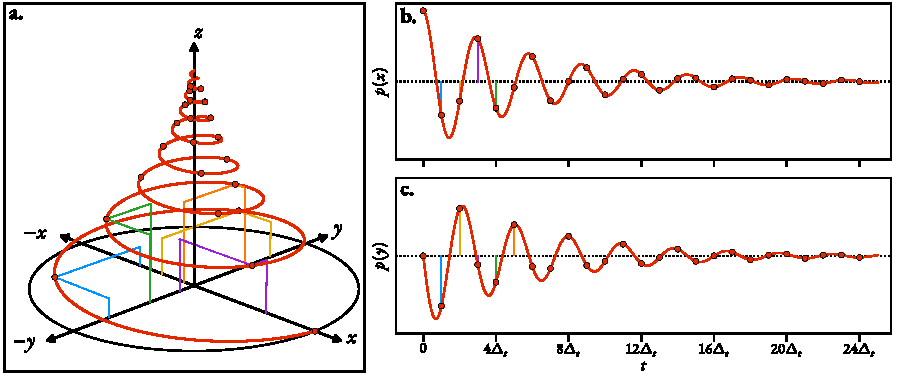
\includegraphics{quadrature_detection/quadrature_detection.pdf}
    \caption[
        An illustration of the free evolution of the bulk
        magnetisation of an ensemble of spin-$\nicefrac{1}{2}$ nuclei
        according to the Bloch model.
    ]{
        \textbf{a.} An illustration of the free evolution of the bulk
        magnetisation of an ensemble of spin-$\nicefrac{1}{2}$ nuclei
        immediately after the application of a $\ang{90}_y$ pulse according to
        the Bloch model. The rate of transverse relaxation was set to be double
        that of longitudinal relaxation ($T_2 = \nicefrac{T_1}{2}$).
        The projections of the magnetisation vector onto the
        $x$- and  $y$-axes are plotted in panels \textbf{b.} and \textbf{c.},
        respectively. Modern \acs{NMR} spectrometers utilise quadrature
        detection, such that the $x$- and  $y$- projections of the time-varying
        magnetisation are sampled at regular time intervals, separated by
        $\Dt$.  The resulting \acs{FID} is given by the complex value $p(x) +
        \iu p(y)$.
    }\label{fig:quadrature}
\end{figure}

Everything has now been established to state the Bloch equations, which
describe the evolution of the bulk magnetisation of an ensemble of identical
spin-$\nicefrac{1}{2}$ nuclei in the rotating frame:
\begin{equation}
    \frac{\mathrm{d}\tilde{\symbf{M}}(t)}{\mathrm{d}t} =
    \begin{bmatrix}
        -R_2 & -\Omega & -\gamma B_1 \sin(\phi_{\text{RF}}) \\
        \Omega & -R_2 & \gamma B_1 \cos(\phi_{\text{RF}}) \\
        \gamma B_1 \sin(\phi_{\text{RF}}) & -\gamma B_1 \cos(\phi_{\text{RF}}) & -R_1
    \end{bmatrix}
    \tilde{\symbf{M}}(t)
    + R_1 M_0
    \begin{bmatrix}
        0 \\ 0 \\ 1
    \end{bmatrix},
\end{equation}
\Cref{fig:quadrature}.a depicts the
evolution of a bulk magnetisation vector after the application of an
\ac{RF} pulse with $\phi_{\text{RF}} = \nicefrac{\pi}{2}$, and an appropriate
combination of duration and power to induce a clockwise rotation of \ang{90}
about the $y$-axis; such a pulse is denoted $\ang{90}_{y}$.
Assuming that negligible evolution due to the offset occurs during the pulse,
the magnetisation vector will land on the $x$-axis, and evolve according to
\begin{subequations}
    \begin{gather}
        \tilde{M}_x(t) = M_0 \cos(\Omega t) \exp(-R_2 t),\\
        \tilde{M}_y(t) = M_0 \sin(\Omega t) \exp(-R_2 t),\\
        \tilde{M}_z(t) = M_0 (1 - \exp(-R_1 t)),
    \end{gather}
\end{subequations}
with $t=\qty{0}{\second}$ denoting the time that the magnetisation lands on the
$x$-axis.
During acquisition, the transverse components of the bulk magnetisation are
detected by the spectrometer probe circuitry
(Figures \ref{fig:quadrature}.b and \ref{fig:quadrature}.c), such that the
resulting signal, called the \acfi{FID}, is given by
\begin{subequations}
    \begin{gather}
        y(t) = c \tilde{M}_+(t),\\
        \tilde{M}_+(t) = \tilde{M}_x (t) + \iu \tilde{M}_y (t) = M_0 \exp(\iu \Omega t - R_2 t),
    \end{gather}
\end{subequations}
with $c \in \mathbb{R}_{>0}$ being a proportionality constant.


\subsection{The NMR Spectrometer}

Modern \ac{NMR} spectrometers are capable of conducting a plethora of
experiments which can aide chemists.
In essence, a spectrometer comprises a high-field magnet, a probe, components
which are used to transmit \ac{RF} pulses to the probe, and components which
are used to process the resulting signal from the probe. A brief summary of
these is now given.

\subsubsection{The Magnet}
The static $\symbf{B}_0$ field is generated by a magnet which is composed of a
superconducting solenoid immersed in liquid helium; common materials used for
the solenoid include Nb-Ti alloy and Nb\textsubscript{3}Sn. To minimise the
extent of helium evaporation, the dewar containing the helium is lined with
a thermal radiation shield. The helium dewar is then surrounded by a larger
dewar containing liquid nitrogen,
\correction{which is finally encased in a vacuum chamber.\label{corr:vacuum}}
A bore passes through the $z$-direction of
the magnet, which is maintained at a user-specified temperature. Within the
bore sits the probe as well as the sample. Magnets with high field
strengths are desirable, as both the resolution ($\propto B_0$) and \ac{SNR}
($\propto B_0^{\nicefrac{3}{2}}$) of the data are affected. At the
time of writing, commercial spectrometers which operate at and above a
\proton\ Larmor frequency of \qty{1}{\giga\hertz} (\qty{23.5}{\tesla}) exist,
though these are uncommon and are employed primarily for the study of large
biomolecules
\correction{and solid-state \ac{NMR}\label{corr:solid-state}}.
For most applications, including
the study of small molecules, spectrometers with more modest field strengths on
the order of \qty{100}{\mega\hertz} are typically adequate. Due to their cheap
operating costs and small size, ``benchtop'' \ac{NMR} spectrometers, which
comprise permanent magnets and typically operate on the order of
\qty{10}{\mega\hertz}, have also become popular in educational and
high-throughput settings~\cite{Giberson2021}.

To ensure a high spatial field homogeneity (a necessity for data with
acceptable resolution) a series of coils called \textit{shims} surround the
sample. Each coil produces a weak magnetic field with a specific spatial
profile in accordance with a spherical harmonic function; a collection of shims
can cancel out
\correction{small\label{corr:small-inhomog}}
inhomogeneities inherent to the main magnet.
A field-frequency lock is used to ensure the stability of the
field. The lock is effectively a small \ac{NMR} spectrometer, tuned to a
specified isotope (typically \textsuperscript{2}H\footnote{
    \textsuperscript{2}H-enriched solvents are routinely used to make up
    \ac{NMR} samples. In \proton\ \ac{NMR} experiments, this ensures that an
    extremely intense signal due to the solvent does not dwarf the signals from
    other spins in the sample. This makes \textsuperscript{2}H a suitable
    nucleus to monitor by the lock, as it present in high concentrations, but
    rarely directly studied.
}), which monitors the resonance frequency of the isotope over
time. If the frequency begins to drift, the current in the $Z_0$ coil is
appropriately adjusted, which induces a constant change in field strength
throughout the sample volume.

\subsubsection{The Probe}
\correction{The probe sits inside the bore of the magnet and has a number of
responsibilities including holding the sample, regulating the sample temperature,
and housing the coils used to pulse the sample with \ac{RF}
radiation as well as coils which are used to generate field
gradients\cite[Section 4.7]{Levitt2007}.\label{corr:probe}}
The \ac{RF} coils also receive the response from the sample during detection.
The principle source of data corruption in \ac{NMR} experiments is thermal
noise within the probe circuitry.  For this reason, cryogenic probes have
become a popular development, in which the coils and other probe electronics
are maintained at a very low temperature (typically about
$\qty{20}{\kelvin}$)~\cite{Kovacs2020}.

\subsubsection{The Transmitter}
The transmitter is responsible for the generation of \ac{RF} pulses
with specified power, timing and phase.
A synthesiser acts as an \ac{RF} source, producing a continuous carrier wave at
or very close to the Larmor frequency of the target nucleus. This frequency
($\omega_{\text{RF}}$) can be adjusted in order to determine the center of the
spectrum. The difference between the carrier frequency and the reference
``basic frequency'' of the spectrometer is referred to as the \emph{transmitter
offset} $\foff$.  The output of the synthesiser is gated to ensure pulses are
applied at the desired times. Attenuators/amplifiers then adjust the power
of the pulse, which travels to the probe.

\subsubsection{The Receiver}
During detection, the time-varying current induced in the probe coil by
the sample magnetisation \correction{travels to\label{corr:travel}} a receiver,
which comprises a series of components designed to convert the
analogue current to the digital \ac{FID} which is stored in computer memory.
One of the processes that the receiver is responsible for is \emph{quadrature
detection}~\cite[Section 13.6]{Keeler2010}, which ensures
\acp{FID} are frequency discriminated, i.e. that they possess the requisite
information to determine whether a given component in the \ac{FID} has a
frequency that is above or below the transmitter frequency.
This is achieved by splitting the signal from the probe into two channels. In
each channel, the signal, which is of a very high frequency
(\unit{\mega\hertz}), is mixed with a reference signal of frequency
$\omega_{\text{RF}}$. The mixing process results in a low-frequency
(\unit{\kilo\hertz}) signal being generated, along with a very high frequency
signal. The reference signal in one channel possesses a phase which
is shifted by \ang{90} relative to the other, such that the combined signal
constitutes a quadrature pair.
Both signals are then sent through a low-pass filter to remove
the high frequency component produced through mixing. Finally, an analogue to
digital converter translates the signal to the real and imaginary components of
a binary dataset which constitutes the \ac{FID}.

\subsection{The Structure of the \acs{FID}}
The result of running a \ac{1D} \ac{NMR} experiment is an \ac{FID} $\by \in
\mathbb{C}^N$ which is sampled at equally spaced points in time, with
consecutive samples separated by time $\Dt$:
\begin{equation}
    \begin{gathered}
        \by = \begin{bmatrix}
            y_0 & y_1 & y_2 & \cdots & y_{N-1}
      \end{bmatrix}\T\\
      \equiv
      \begin{bmatrix}
          y(t=0) & y(t=\Dt) & y(t=2\Dt) & \cdots & y(t=(N-1)\Dt)
      \end{bmatrix}\T,
    \end{gathered}
\end{equation}
where $y(t)$ is the (continuous) variation of the generated signal as a
function of time,
and $N$ (often a power of 2) is the number of points sampled. The inverse of
the sampling rate,
$\nicefrac{1}{\Dt}$ is the \correction{\emph{spectral width}\label{corr:sw}} $\fsw$ which
defines how wide the range of samplable frequencies is, in accordance with the
Nyquist theorem~\cite{Shannon1949}.

\acp{FID} adopt the form of a summation of $M \in \mathbb{N}$ complex
exponentials (signals). Each signal will be subjected to damping due to
transverse relaxation, which is typically exponential in nature. An \ac{FID}
therefore takes the form\footnote{
    \correction{
        This provides an idealised model of an \ac{FID}, based on the
        underlying theory of the experiment. In reality, there is the possibility
        of significant deviations from this model being realised. One potential
        cause of this is the influence of magnetic field inhomogeneities, which
        will cause spectral peaks to deviate from having Lorentzian lineshapes
        (\cref{subsec:nmr-proc}). In cases where distortions to the data have
        occurred, techniques such as \emph{reference deconvolution}~\cite{Morris1997}
        can be used as a corrective measure in a bid to make the data agree more
        closely with this model.
    }\label{fn:ref-decon}
}
\begin{subequations}
    \begin{gather}
        y_n = x_n(\bth) + w_n \quad
            \quad \forall n \in \lbrace 0, 1, \cdots, N - 1 \rbrace,
            \label{eq:y=x+w} \\
        x_n(\bth) =
        \sumM \amexpphim \exp\left(
            (2 \pi \iu (f_m - \foff)- \eta_m ) n \Dt
        \right).
        \label{eq:x-1d}
    \end{gather}
    \label{eq:1d}%
\end{subequations}%
\cref{eq:1d} indicates that \iac{FID} comprises contributions from the
(deterministic) evolution of the spin magnetisation $\bx$ and experimental
noise $\bw$ (\emph{vide infra}). Each signal which contributes to $\bx$ is
defined by four parameters:
\begin{itemize}
    \item Amplitude $a \in \mathbb{R}_{>0}$ ,
    \label{pg:param-constraints}
    \item Phase $\phi \in (-\pi, \pi]$ (\unit{\radian}),
    \item Frequency $f \in \left[\hspace*{2pt}\foff - \nicefrac{1}{2} \hspace*{2pt}
        \fsw, \foff + \nicefrac{1}{2} \hspace*{2pt}\fsw \right]$ (\unit{\hertz}),
    \item Damping factor $\eta \in \mathbb{R}_{>0}$ (\unit{\per\second}).
\end{itemize}%
\Iac{FID} can therefore be parameterised by the vector $\bth \in
\mathbb{R}^{4M}$:
\begin{equation}
    \bth =
    \begin{bmatrix}
        \symbf{a}\T & \symbf{\phi}\T & \symbf{f}\T & \symbf{\eta}\T
    \end{bmatrix}\T,
\end{equation}
where $\bda \in \mathbb{R}^M = [a_1 \hspace{2pt} a_2 \hspace{2pt} \cdots
\hspace{2pt} a_M]^{\mathrm{T}}$ is a vector of all amplitudes, $\bdphi \in
\mathbb{R}^M$ is a vector of all phases, etc.
A more concise alternative to \correction{\cref{eq:x-1d}}
involves the \emph{complex amplitudes} and \emph{signal poles} associated with
the \ac{FID}:
\begin{subequations}
    \begin{gather}
        x_n(\bth) = \sumM \alpha_m^{\vphantom{n}} z_m^n,\\
        \alpha_m = \amexpphim,\\
        z_m = \exp\left(
            \left(2 \pi \iu \left(f_m - \foff\right) - \eta_m\right) \Dt
        \right).\label{eq:signal-pole}
    \end{gather}
    \label{eq:x-alpha-z}%
\end{subequations}
The respective influences of the four parameters on a signal in the time-domain
are depicted in Figures \ref{fig:amp-phase-freq-damp}.a1 to
\ref{fig:amp-phase-freq-damp}.d1.
\begin{figure}
    \centering
    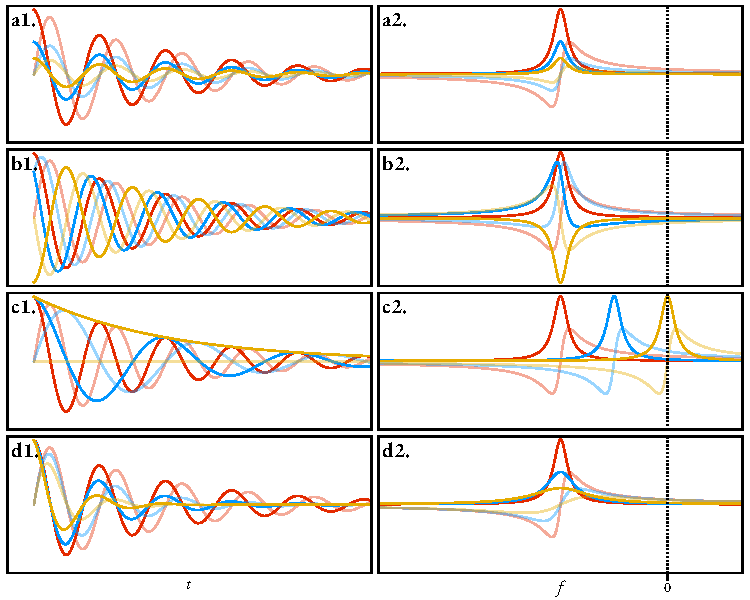
\includegraphics{amp_phase_freq_damp/amp_phase_freq_damp.pdf}
    \caption[
        An illustration of the influence of the four parameters associated
        with a signal in both the time-domain and the Fourier-domain.
    ]{
        An illustration of the influence of the four parameters associated
        with a signal in both the time-domain (a1 to d1) and Fourier-domain
        (a2 to d2).
        The red signal is generated with the same parameters across all panels:
        $a = a_{\text{red}}$, $\phi = 0\,\unit{\radian}$, $f = f_{\text{red}}$,  $\eta =
        \eta_{\text{red}}$.  The blue and yellow signals were produced by
        altering one parameter out of the four.
        \textbf{a.} $a_{\text{yellow}} = \nicefrac{1}{2} a_{\text{blue}} =
        \nicefrac{1}{4} a_{\text{red}}$.
        \textbf{b.}
        $\phi_{\text{blue}} = \nicefrac{\pi}{4}\,\unit{\radian}$,
        $\phi_{\text{yellow}} = \pi\,\unit{\radian}$.
        \textbf{c.}
        $f_{\text{blue}} = \nicefrac{1}{2} f_{\text{red}}$,
        $f_{\text{yellow}} = 0$.
        \textbf{d.}
        $\eta_{\text{yellow}} =
        \nicefrac{1}{2}\eta_{\text{blue}} =
        \nicefrac{1}{4}\eta_{\text{red}}$.
        The real and imaginary components of each signal are plotted, with the
        imaginary component being paler than its real counterpart.
    }
    \label{fig:amp-phase-freq-damp}%
\end{figure}

Multidimensional experiments involve incrementing one or more delays within the
pulse sequence, in order to obtain an array of \ac{1D} \acp{FID}. In a
$D$-dimensional dataset, each contributing signal is parameterised by an
amplitude and phase as before, along with $D$ distinct frequencies and damping
factors, such that a general parameter vector  $\bth \in \mathbb{R}^{2(1+D)M}$
is given by
\begin{equation}
    \bth =
    \begin{bmatrix}
    \symbf{a}\T &
    \symbf{\phi}\T &
    {\bdfone}\T &
    \cdots &
    {\bdfD}\T &
    {\bdetaone}\T &
    \cdots &
    {\bdetaD}\T
    \end{bmatrix}\T,
    \label{eq:theta}
\end{equation}
where $\bdfD$ and $\bdetaD$ are the frequencies and damping factors in the
actively acquired (direct) dimension, and $\lbrace \bdfone, \cdots,
\bdfDminusone \rbrace$ and
$\lbrace \bdetaone, \cdots, \bdetaDminusone \rbrace$ are those for the indirect
dimension(s).
Indirect dimensions can exhibit different forms of evolution, depending on
the precise nature of the pulse sequence, of which two are very
common~\cite[Section 4.3.4]{Cavanagh2007}. \acp{FID} whose constituent signals
evolve according to $\cos(2 \pi f t)$ or $\sin(2 \pi f t)$ modulate the
amplitude of the direct dimension across increments, while those whose signals
evolve according to $\exp(2 \pi \iu f t)$ and $\exp(-2 \pi \iu f t)$ modulate
the phase instead.
For experiments which produce amplitude-modulated \acp{FID},
both the cosine and sine forms should be acquired if possible, as this ensures
that spectra with desirable properties can be generated. The same is true for the positive
and negative forms when phase-modulated \acp{FID} are acquired (\emph{vide
infra}). In general, a $D$-dimensional \ac{FID} $\bY \in \mathbb{C}^{\None
\times \cdots \times \ND}$ can be expressed as
\begin{subequations}
    \begin{gather}
        \ynonenD = \xnonenD(\bth) + \wnonenD,\\
        \xnonenD
            = \sumM \amexpphim \prodD
            \zeta^{(d)}\left(2 \pi \left(f^{(d)}_m  - \foffd\right) \nd \Dtd\right)
            \exp\left(-\eta^{(d)}_m \nd \Dtd\right),\\
        \zeta^{(d)}(\cdot)
        \begin{cases}
            = \exp(\iu\cdot) & d = D \\
            \in \left\lbrace \cos(\cdot), \sin(\cdot), \exp(\iu\cdot) \exp(-\iu\cdot)\right\rbrace & \text{otherwise}
        \end{cases},
    \end{gather}
    \label{eq:general-fid}%
\end{subequations}%

It is typical to assume that the data is corrupted by an array of \ac{AWGN},
i.e. the noise instances are described by a complex normal distribution with
mean 0, and pairs of noise instances are statistically independent, regardless
of their time separation:
\begin{subequations}
    \begin{gather}
        \wnonenD \sim
        \mathcal{N_C}\left(0, 2\sigma^2\right) \\
        \begin{gathered}
            \implies \Re\left(\wnonenD\right) \upmodels \Im\left(\wnonenD\right),\\
             \Re\left(\wnonenD\right) \sim \mathcal{N}\left(0, \sigma^2\right),\\
             \Im\left(\wnonenD\right) \sim \mathcal{N}\left(0, \sigma^2\right). \\
        \end{gathered}
    \end{gather}
\end{subequations}
The extent by which \iac{FID} is corrupted by noise is given by its \ac{SNR},
the ratio of signal power and noise power:
\begin{equation}
    \SNR\left(\bY\right) \coloneq
        \frac{1}{2 N_{\text{tot}} \sigma^2}
        \sum_{\none=0}^{\None-1} \cdots \sum_{\nd=0}^{\ND-1}
        \left \lvert \xnonenD \right \rvert^2,
        \label{eq:snr}
\end{equation}
where $N_{\text{tot}} \coloneq \None \times \cdots \times \ND$ is the total
number of points the \ac{FID} comprises. Due to the large dynamic range
observed for the \ac{SNR} across datasets, it is common to express it using a
logarithmic scale instead, in units of decibels (\unit{\deci\bel}):
\begin{equation}
    \SNR_{\unit{\deci\bel}} \coloneq 10 \log_{10} \left(\SNR\right).
    \label{eq:snr-db}
\end{equation}
